% Created 2020-09-24 Thu 17:24
% Intended LaTeX compiler: pdflatex
\documentclass[11pt]{article}
\usepackage[utf8]{inputenc}
\usepackage[T1]{fontenc}
\usepackage{graphicx}
\usepackage{grffile}
\usepackage{longtable}
\usepackage{wrapfig}
\usepackage{rotating}
\usepackage[normalem]{ulem}
\usepackage{amsmath}
\usepackage{textcomp}
\usepackage{amssymb}
\usepackage{capt-of}
\usepackage{hyperref}
\author{Alex Day}
\date{\today}
\title{Artificial Intelligence}
\hypersetup{
 pdfauthor={Alex Day},
 pdftitle={Artificial Intelligence},
 pdfkeywords={},
 pdfsubject={},
 pdfcreator={Emacs 27.1 (Org mode 9.4)}, 
 pdflang={English}}
\begin{document}

\maketitle
\tableofcontents


\section{AI Basics}
\label{sec:org63f78e3}
\subsection{Agents}
\label{sec:org9482631}
\begin{itemize}
\item An \textbf{agent} is an entity that perceives and acts
\item A \textbf{rational agent} selects actions that achieve the best (expected) outcome
\item \textbf{Reflex agents} consider how the world is but do \textbf{\textbf{not}} consider future consequences of their actions
\begin{itemize}
\item Can sometimes be rational, although not always
\end{itemize}
\item \textbf{Planning agents} consider how the world would be based upon their actions and have some goal
\begin{itemize}
\item Decisions are based on hypothesized consequences of actions
\item Not always the \textbf{\textbf{best}} action so they're note always rational
\end{itemize}
\end{itemize}

\subsection{Searching}
\label{sec:org5e3dee1}
\begin{itemize}
\item In a Discrete Search Problem we are given:
\begin{itemize}
\item A finite state space
\item A finite action space
\item A cost function
\begin{itemize}
\item \(Cost=C(Action, State, FutureState)\)
\item The cost of an action is defined as the cost of moving from a state to some future state through that action
\end{itemize}
\item A transition model
\begin{itemize}
\item \(FutureState=Transition(Action, CurrentState)\)
\end{itemize}
\item Start state and a goal state or goal test
\item We seek to find a minimum cost solution solution: a sequence of actions that lead from the start to the goal
\item We assume the cost of the solution is equal to the sum of the cost of each step
\end{itemize}
\end{itemize}

\subsection{State Space Graphs vs Search Trees}
\label{sec:orge69a0c8}
\begin{itemize}
\item State Space Graphs
\begin{itemize}
\item The state space forms a directed graph where the nodes are states and the edges are actions
\item Each state occurs only once
\item Goal test is a set of nodes
\item Rarely can build it in memory
\end{itemize}
\item Search Trees
\begin{itemize}
\item Root has the start state
\item Branches are actions
\item The nodes show states but correspond to local PLANS
\item Search trees can be expanded until the solution is found
\begin{itemize}
\item Leaf nodes are called the frontier or the open list
\item Leaf nodes are nodes that have unexplored options
\end{itemize}
\end{itemize}
\end{itemize}

\section{Uninformed Search}
\label{sec:orgbf5dc53}
\subsection{Breadth First Search}
\label{sec:orgd1b18ff}
\begin{itemize}
\item Expand shallowest node first
\item Frontier is a FIFO queue
\end{itemize}

\subsection{Depth First Search}
\label{sec:org5e33f20}
\begin{itemize}
\item Always expand the deepest node first
\item Frontier is a LIFO queue (stack)
\end{itemize}

\subsection{Iterative Deepening}
\label{sec:org63b695a}
\begin{itemize}
\item Run DFS with depth limit 1
\item Run DFS with depth limit 2
\item Run DFS with depth limit \ldots{}
\item DFS space complexity with BFS time complexity
\end{itemize}

\subsection{Uniform Cost Search}
\label{sec:org4e7705b}
\begin{itemize}
\item Expand least-cost node first
\item Frontier is a priority queue
\item Issues
\begin{itemize}
\item Explores in all directions
\item No goal-oriented expansion
\end{itemize}
\end{itemize}

\subsection{Search Algorithm Evaluation}
\label{sec:orgda1b6e8}
\begin{itemize}
\item Completeness - Does this always find a solution if one exists
\item Optimal - Find the least cost solution
\item Time complexity - Time taken
\item Space complexity - Space needed
\item Useful quantities
\begin{itemize}
\item \(b\) - branching factor of the tree (average number of successors for any node)
\item \(m\) - Maximum depth of the state space (meaning there are at max \(b^m\) nodes)
\item \(d\) - Depth of the shallowest goal node
\begin{center}
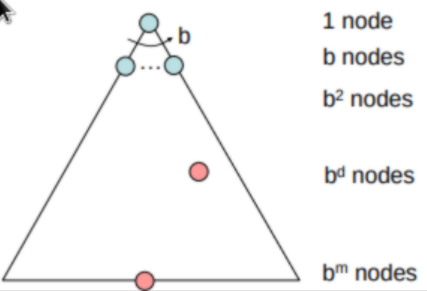
\includegraphics[width=.9\linewidth]{images/2020-09-03_16-49-29_screenshot.png}
\end{center}
\end{itemize}
\end{itemize}
\subsubsection{BFS Properties}
\label{sec:org3f4afe1}
\begin{itemize}
\item Time complexity \(\approx O(b^d)\)
\item Space complexity \(\approx O(b^d)\)
\item It is complete (if \(d\) is finite)
\item It is optimal only if step costs are equal or increasing as we move down the tree
\item BFS requires a crazy amount of memory and time
\end{itemize}
\subsubsection{DFS Properties}
\label{sec:org2fbf8a8}
\begin{itemize}
\item It is complete if \(m\) is finite and the graph is acyclic
\item Not optimal
\item Time complexity \(O(b^m)\) if \(m \ne \infty\) and terrible if \(m >> d\)
\item Space complexity \(O(bm)\)
\end{itemize}
\subsubsection{UCS properties}
\label{sec:org5fc0046}
\begin{itemize}
\item It is optimal
\item It is complete if the cost of every action is at least \(\epsilon > 0\)
\item Time
\begin{itemize}
\item If \(C^*\) is the optimal cost the effective depth is \(\frac{C^*}{\epsilon}\)
\item It takes \(O(b^{\frac{C^*}{\epsilon}})\) time and space
\end{itemize}
\end{itemize}
\section{Informed Search}
\label{sec:orgd4adeff}
\begin{itemize}
\item \textbf{Informed Search Methods} use problem specific knowledge to solve a problem better
\item \textbf{Idea}: Use an \emph{evaluation} function \(f(n)\) for each node \(n\)
\begin{itemize}
\item Estimate ``desirability'' of each node
\end{itemize}
\item Open is a priority queue sorted by increasing \$f\$-cost
\end{itemize}

\subsection{Search Heuristic}
\label{sec:orgca1dd3d}
\begin{itemize}
\item A heuristic function \(h(n)\)
\begin{itemize}
\item Estimates how close the state at node \(n\) is to the goal state
\item Designed for a particular search problem
\item Common heuristics: Manhattan distance, Euclidean distance, etc.
\end{itemize}
\end{itemize}

\subsection{Greedy Search}
\label{sec:orgbabcf12}
\begin{itemize}
\item Expand the node that appears to be closest to the goal at each step
\item \(f(n)=h(n)\)
\item Complete
\item Not Optimal
\item Time - \(O(b^m)\)
\item Space - \(O(b^m)\)
\end{itemize}

\subsection{A*}
\label{sec:org766b735}
\begin{itemize}
\item Guide the search while avoid expanding expensive paths
\item Evaluation function \(f(n)  = g(n) + h(n)\)
\item Admissible heuristics
\begin{itemize}
\item Never overestimate true cost of the goal
\end{itemize}
\item Consistent heuristics
\begin{itemize}
\item \(h(n) <= c(n, a, n')+h(n')\)
\item Where \(c\) is a step cost function
\item All consistent heuristics are admissible
\end{itemize}
\item Most of the work in A* lies on finding admissible heuristics
\begin{itemize}
\item We can often find these by solving a \emph{relaxed} version of the problem
\begin{itemize}
\item The \textbf{key} idea is the optimal solution cost of the relaxed problem is no greater than the optimal solution cost of the real problem
\end{itemize}
\end{itemize}
\item Given two heuristics \(h_1\) and \(h_2\) if \(h_{2}(n) >= h_{1}(n) \forall n\) then \(h_2\) \textbf{dominates} \(h_1\) and is better for search
\item Given \(m\) admissible heuristics \(h_1, h_2, \dots, h_3\) then \(h(n) = max(h_1(n), h_2(n), \dots, h_n(n))\) is also admissable and dominates any \(h_i\)
\item A* has extensions that allow incremental, anytime, and pruning approahces
\end{itemize}

\section{Probabilities}
\label{sec:org24bb434}
\begin{itemize}
\item A random variable \(X\), represents an event whose outcome is unknown
\item \(P\) is a probability distribution that assigns weight to outcomes
\begin{itemize}
\item \(X=\) weather tomorrow
\item \(X \in \{sunshine, rain, thunder\}\)
\item \(P(X=sunshine)=0.5\), \(P(X=rain) = 0.25\), \(P(X=thunder) = 0.25\)
\end{itemize}
\item Probabilities are non-neg and sum to one
\item As we get more evidence the probabilities may change
\item The \textbf{expected value}, \(E\), of a function of a random variable is the average, weighted by the probability distribution over outcomes
\end{itemize}
\section{Markov Decision Process}
\label{sec:orgcd64e13}
\subsection{Stochasticity}
\label{sec:org1c177f8}
\begin{itemize}
\item Sometimes you cannot rely that a given action from a specific state may always take you to a certain state
\item How can we act optimally in the face of randomness
\end{itemize}
\subsection{Gridworld}
\label{sec:orgb357dd0}
\begin{itemize}
\item Noisy motion model
\begin{itemize}
\item 80\% the action N takes the agent North (if there is no wall)
\item 10\% N goes West, 10\% N goes east
\item If there is a wall the agent stays put
\end{itemize}
\item The agent receives rewards at each step and a big reward if it exits at +1 and a bad reward if it exits at -1
\begin{center}
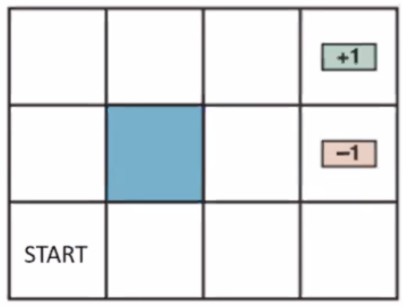
\includegraphics[width=.9\linewidth]{images/2020-09-03_17-54-54_screenshot.png}
\end{center}
\end{itemize}
\subsection{Stochastic motion model}
\label{sec:org61c2e1b}
\begin{center}
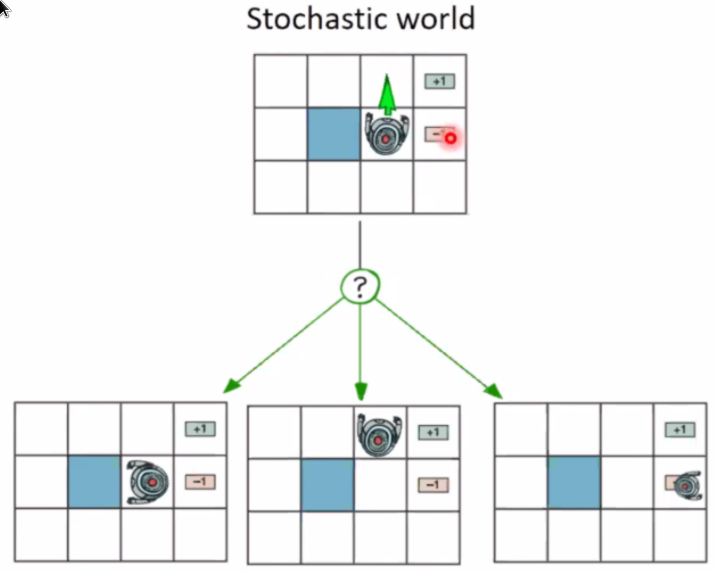
\includegraphics[width=.9\linewidth]{images/2020-09-03_17-58-54_screenshot.png}
\end{center}

\subsection{Simple Game}
\label{sec:orgb273905}
\begin{itemize}
\item At each round:
\begin{enumerate}
\item Stay or quit
\item If quit: you get \$10
\item If stay: you get \$5 and then roll a die
\begin{enumerate}
\item If the result is 1 or 2 the game ended
\item Otherwise the game continues to the next round
\end{enumerate}
\end{enumerate}
\end{itemize}
\begin{center}
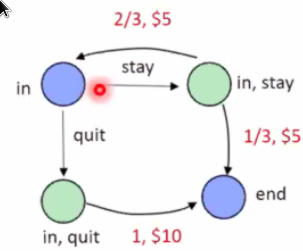
\includegraphics[width=.9\linewidth]{images/2020-09-03_18-02-27_screenshot.png}
\end{center}
In a Markov Decision Process there are state nodes (in blue), chance nodes (in green), choice edges (in black text), and reward edges with the probability and reward (in red)
\subsection{Markov Decision Process}
\label{sec:org36721cd}
\begin{itemize}
\item A set of states \(S\)
\item A set of actions \(A\)
\item A transition function \(T(s, a, s')\)
\begin{itemize}
\item Also called the model or dynamics
\item Sometimes \(P(s'|s, a)\)
\end{itemize}
\item A reward function \(R(s, a, s')\)
\begin{itemize}
\item Sometimes just \(R(s)\) or \(R(s')\)
\item A start state \(s_0\) (and maybe a terminal state)
\end{itemize}
\item MDPs are non-deterministic search problems
\begin{center}
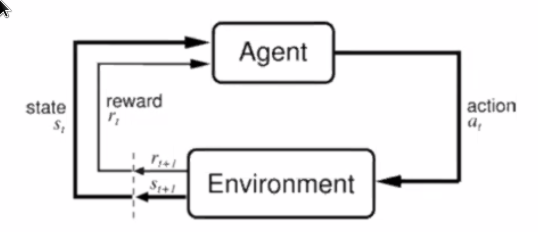
\includegraphics[width=.9\linewidth]{images/2020-09-03_18-05-59_screenshot.png}
\end{center}
\item In a MDP, ``Markov'' means that the action outcomes depend only on the current state
\begin{center}
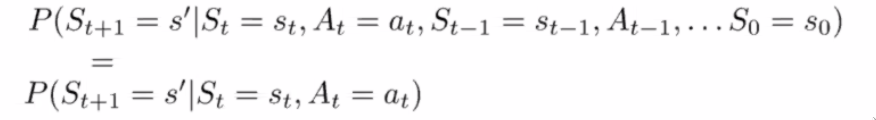
\includegraphics[width=.9\linewidth]{images/2020-09-03_18-07-52_screenshot.png}
\end{center}
\item This is just like search: in the 1st assignment the children of an expanded state depended only on the current node not how you got there
\end{itemize}
\subsection{Policy}
\label{sec:org1a78a40}
\begin{itemize}
\item In deterministic we seek an optimal sequence of actions from start to goal
\item In stochastic we seek an optimal policy \(\pi^*:S \rightarrow A\)
\begin{itemize}
\item Policy \(\pi\) gives an action for each state
\end{itemize}
\item Following a policy yields a random path
\item The utility, \(U\), of a policy is the (discounted) sum of the rewards along the path
\item The goal is to find an optimal policy, \(\pi^*\) that maximizes the expected utility
\end{itemize}
\subsection{Discounting}
\label{sec:org1ca20cc}
\begin{itemize}
\item It's reasonable to maximize the sum of rewards
\item It's also reasonable to prefer rewards now to rewards later
\item Solution: values of rewards decay exponentially over time based on some discount factor \(0 <= \gamma <= 1\)
\item We discount so that algorithms can converge and have theoretical guarantees
\end{itemize}
\subsection{Avoiding Infinite Rewards}
\label{sec:orgaa4a59c}
\begin{itemize}
\item \textbf{Problem}: If the game lasts forever, do we get infinite rewards?
\item Solutions:
\begin{itemize}
\item Introduce some artificial time horizon \(H\)
\begin{itemize}
\item Gives nonstationary policies (\(\pi\) depends on the time left)
\end{itemize}
\item Discounting: use \(0< \gamma <1\)
\item Absorbing state: guarantee that for every policy a terminal state will eventually be reached
\end{itemize}
\end{itemize}
\subsection{Revisitng MDPs}
\label{sec:org74fec8a}
\begin{itemize}
\item Same definition as before but with:
\begin{itemize}
\item Discount factor \(\gamma\)
\item Horizon \(H\) (can be \(\infty\))
\end{itemize}
\item MDP quantities so far
\begin{itemize}
\item Policy \(\pi\): Choice of action for each state
\item Utility \(U_\pi=\Sigma^H_{t=0}\gamma^tR(s_t)\) Sum of discounte d rewards
\end{itemize}
\end{itemize}
\subsection{Solving MDPs}
\label{sec:org8a0fec3}
\subsubsection{Value Iteration}
\label{sec:org904e045}
\begin{itemize}
\item \(\pi^*=\text{argmax}_\pi \mathbb{E} [\Sigma^H_{t=0}\gamma^tR(s_t) | \pi]\)
\end{itemize}
\begin{enumerate}
\item Optimal value Function \(V^*\)
\label{sec:orgd129447}
\begin{itemize}
\item \(V^*(s)\) is the sum of discounted rewards starting in \(s\) and acting optimally
\end{itemize}
\begin{center}
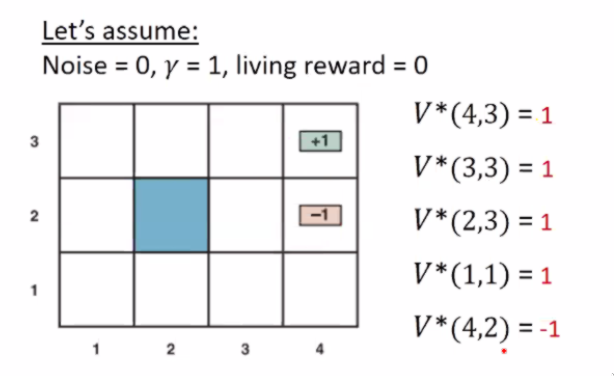
\includegraphics[width=.9\linewidth]{images/2020-09-08_17-31-58_screenshot.png}
\end{center}

\begin{center}
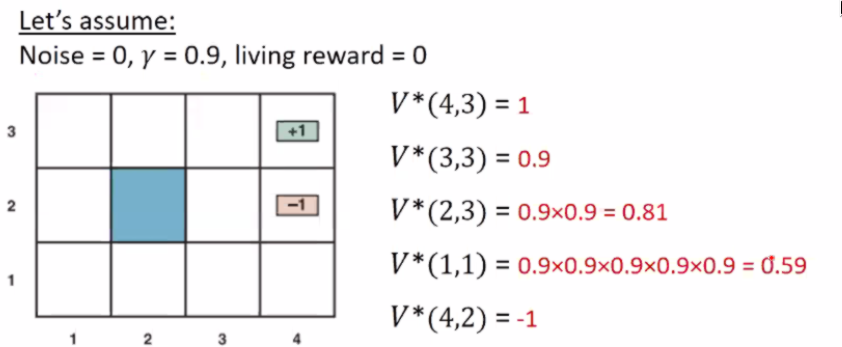
\includegraphics[width=.9\linewidth]{images/2020-09-08_17-34-27_screenshot.png}
\end{center}

\begin{itemize}
\item Closed form for \(V^*\) is CV\(V^*=max_a(R(s, a, s') + \gamma V^*(s'))\)
\begin{center}
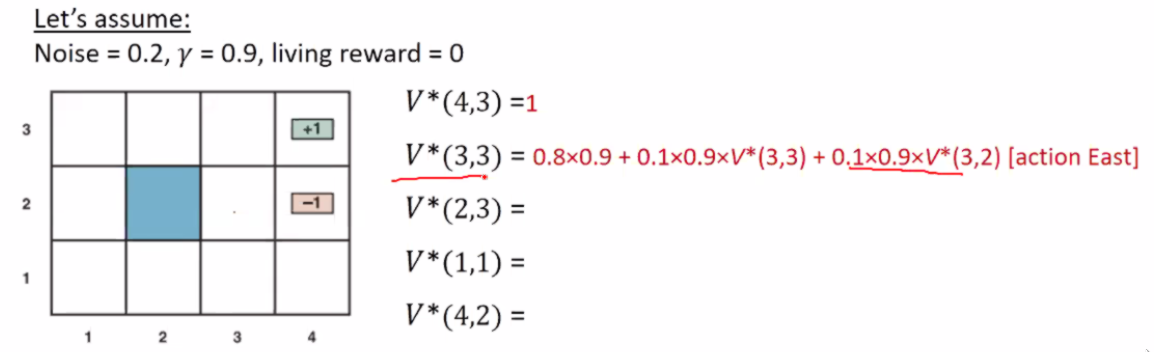
\includegraphics[width=.9\linewidth]{images/2020-09-08_17-40-23_screenshot.png}
\end{center}
\end{itemize}
\item Bellman Equation
\label{sec:orgb32141c}
\(V^*(s) = max_a \mathbb{E} [R(s, a, s') + \gamma V^*(s')]\)
\item Q-Values
\label{sec:orgb628065}
\begin{itemize}
\item \(Q^*(s, a)\) = expected utility starting at state \(s\), taking action \(a\), and then acting optimally
\begin{center}
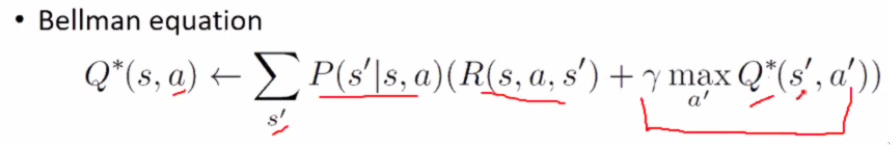
\includegraphics[width=.9\linewidth]{images/2020-09-08_18-06-00_screenshot.png}
\end{center}
\end{itemize}
\end{enumerate}
\subsubsection{Policy Iteration}
\label{sec:orgc437606}
\begin{enumerate}
\item Extracting Policy from \(V^*\)
\label{sec:org541d9d9}
\begin{itemize}
\item It's not obvous
\item We need to keep track of the optimal policy during value iteration
\item This is called policy extraction, since the policy is informed by the value
\end{itemize}
\item Extracting policy from \(Q^*\)
\label{sec:org04c0ce4}
\begin{itemize}
\item Just take the max from each
\item Optimal policy is implicit
\end{itemize}
\item Issues with Value iteration
\label{sec:org5293c44}
\begin{itemize}
\item Slow \(O(S^2A)\) per iteration
\item The ``max'' at each state rarely changes
\item The policy often converges before the actions
\end{itemize}
\item Policy evaluation
\label{sec:org6633f71}
\begin{itemize}
\item In value iteration we max over all actions to compute optimal values
\item If we fixed some policy \(\pi(s)\), then only one action per state
\begin{itemize}
\item \(V^\pi(s)\) =expected total discounted rewards starting in \(s\) and following \(\pi\)
\item The value depends now on which policy we fixed
\end{itemize}
\item Iterate and converge at optimal policy rather than optimal value
\end{itemize}
\end{enumerate}
\section{Reinforcement Learning}
\label{sec:org5503562}
\subsection{Definition}
\label{sec:org22d7c5c}
\begin{itemize}
\item MDP but we don't know \(P\) and \(R\)
\end{itemize}
\subsection{Framework}
\label{sec:org853db48}
At every timestep \(t\) the agent picks an action \(a_t\) and the environment changes to a new state \(s_t\) and the agent is given some reward \(r_t\)
\begin{center}
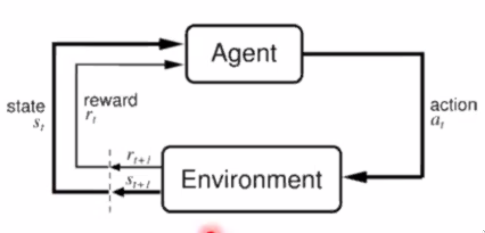
\includegraphics[width=.9\linewidth]{images/2020-09-15_17-13-25_screenshot.png}
\end{center}
\subsection{Model-Based Learning}
\label{sec:orgbe48dbd}
\begin{center}
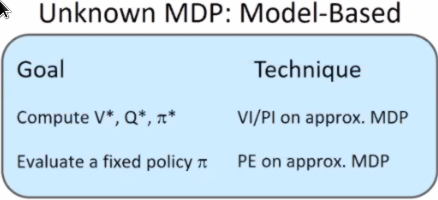
\includegraphics[width=.9\linewidth]{images/2020-09-17_17-13-20_screenshot.png}
\end{center}
\subsubsection{Model-Based Monte Carlo}
\label{sec:org4db55e8}
\begin{enumerate}
\item Learn empirical MDP using Monte Carlo simulation
\begin{enumerate}
\item Episodic data: \(s_0, a_0, r_1, s_1, a_1, ..., s_T\)
\item Estimate transitions and rewards
\begin{center}
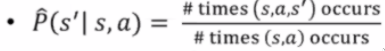
\includegraphics[width=.9\linewidth]{images/2020-09-15_17-19-38_screenshot.png}
\end{center}
\item Discover each \(\hat{R}\) when we experience \((s, a, s')\)
\end{enumerate}
\item Estimates converge to the truth
\item Solve using value/policy iteration
\end{enumerate}
\subsection{Model-Free Learning}
\label{sec:orgb6e401d}
\begin{center}
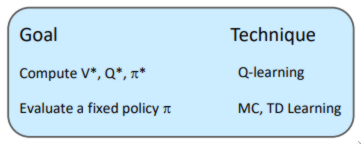
\includegraphics[width=.9\linewidth]{images/2020-09-17_17-14-56_screenshot.png}
\end{center}

\subsubsection{Example}
\label{sec:orgabac939}
\begin{itemize}
\item 
\end{itemize}
\subsection{Q-Learning}
\label{sec:org2e4f2b3}
\begin{itemize}
\item Used to compute \(V^*\), \(Q^*\), and \(\pi^*\) in a model free, unknown MDP
\end{itemize}
\subsubsection{Active RL}
\label{sec:org2636229}
\begin{itemize}
\item Full reinforcement learning
\item Learner makes choices
\item Exploration vs Exploitation
\end{itemize}
\subsubsection{Tabular Q-Learning}
\label{sec:org7d7aa6d}
\begin{itemize}
\item Sample-based Q-value iteration
\begin{center}
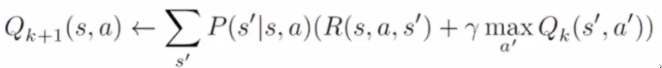
\includegraphics[width=.9\linewidth]{images/2020-09-17_17-26-24_screenshot.png}
\end{center}
\item Learn Q-values as you go
\begin{itemize}
\item Recieve a sample \((s, a, r, s')\)
\item Consider previous estimate \(\hat{Q}(s, a)\)
\item Consider your new sample estimate
\begin{itemize}
\item target \(= R(s,a,s')+\gamma max_{a'}\hat{Q}(s', a')\)
\end{itemize}
\item Incorperate the new estimate into a running average using some learning rate \(\alpha\)
\begin{itemize}
\item \(\hat{Q}(s, a) \leftarrow (1 - a)\hat{Q}(s, a) + \alpha\text{[target]}\)
\end{itemize}
\end{itemize}
\end{itemize}
\subsubsection{Properties}
\label{sec:org38d30b7}
\begin{itemize}
\item Q-learning converges to optimal policy, even if you're acting suboptimally if the policy visits every path
\item This is called off-policy learning
\begin{itemize}
\item On policy: Learn values of the policy used to generate samples
\item Off policy: Learn the value of another policy
\end{itemize}
\item Caveats
\begin{itemize}
\item Lot of exploration
\item Make the learning rate small enough evantually
\item Basically, in the limit, it doesn't matter how you select actions!
\end{itemize}
\end{itemize}
\subsubsection{Exploration vs Exploitation}
\label{sec:orgfb89b01}
\begin{itemize}
\item All states should be visited infinitely often
\item Multi-arm bandit
\end{itemize}
\begin{enumerate}
\item How to sample actions?
\label{sec:orgcb2b0fb}
\begin{itemize}
\item Choose random actions?
\begin{itemize}
\item You need to visit a lot of cells to get enough data of optimal paths
\end{itemize}
\item Choose action greedily?
\begin{itemize}
\item Never try the other paths that could be higher value?
\end{itemize}
\item Answer: start by random and transition to greedy to converge
\item Epsilon-greedy
\begin{itemize}
\item With a (small) probability \(\epsilon\), act randomly
\item With a (large) probability \(1-\epsilon\), act on current policy
\end{itemize}
\end{itemize}
\end{enumerate}
\section{Adversarial Games}
\label{sec:orgbb0eae1}
\subsection{Types of Games}
\label{sec:org5c2c88d}
\begin{itemize}
\item Axes
\begin{itemize}
\item Deterministic vs Stochastic
\item Perfect Information
\item One, two, or more players?
\item Zero sum?
\begin{center}
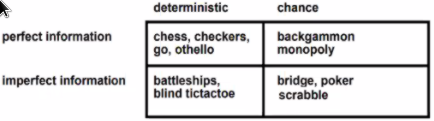
\includegraphics[width=.9\linewidth]{images/2020-09-24_17-13-31_screenshot.png}
\end{center}
\end{itemize}
\end{itemize}

\subsection{Deterministic Games}
\label{sec:org08127af}
\begin{itemize}
\item Search Problem
\begin{itemize}
\item States: \(S\) (starts at \(s_0\))
\item Players: \(P={1\dots N}\)
\item Actions: \(A\)
\item Transition Function \(S \times A \rightarrow S\)
\item Terminal test: \(S \rightarrow \{\text{true},\text{false}\}\)
\item Terminal utilities: \(S \times P \rightarrow \mathbb{R}\)
\end{itemize}
\item Solution for a \emph{player} p is a policy \(\pi_p:S \rightarrow A\)
\begin{itemize}
\item \(\pi_p\) is defined when it is \(p\)'s turn to play
\end{itemize}
\end{itemize}
\subsection{Why are games hard?}
\label{sec:org1b179bf}
\begin{itemize}
\item The utility comes at the end of the game
\item Each state is controlled by different players
\end{itemize}
\subsection{Zero Sum Games}
\label{sec:orgab77ab6}
\begin{itemize}
\item Agents have opposite utilities
\item Single value on maximizes that the other minimizes
\item Adversarial, pure competition
\end{itemize}
\subsection{General Games}
\label{sec:orgc869b9a}
\begin{itemize}
\item Agents have independent utilities
\item Cooperation, indifference, competition, etc.
\end{itemize}
\end{document}
